/section{Modell}
Für die Berechnungen verwenden wir das Modell Park Avenue 432, eines der höchsten reinen Wohnhochhäusern auf der Welt. Die stolze Höhe und der über das ganze Gebäude gleichbleibende quadratische Grundrisses erleichtern unsere Berechnungen. 
\begin{figure}[H]
\centering
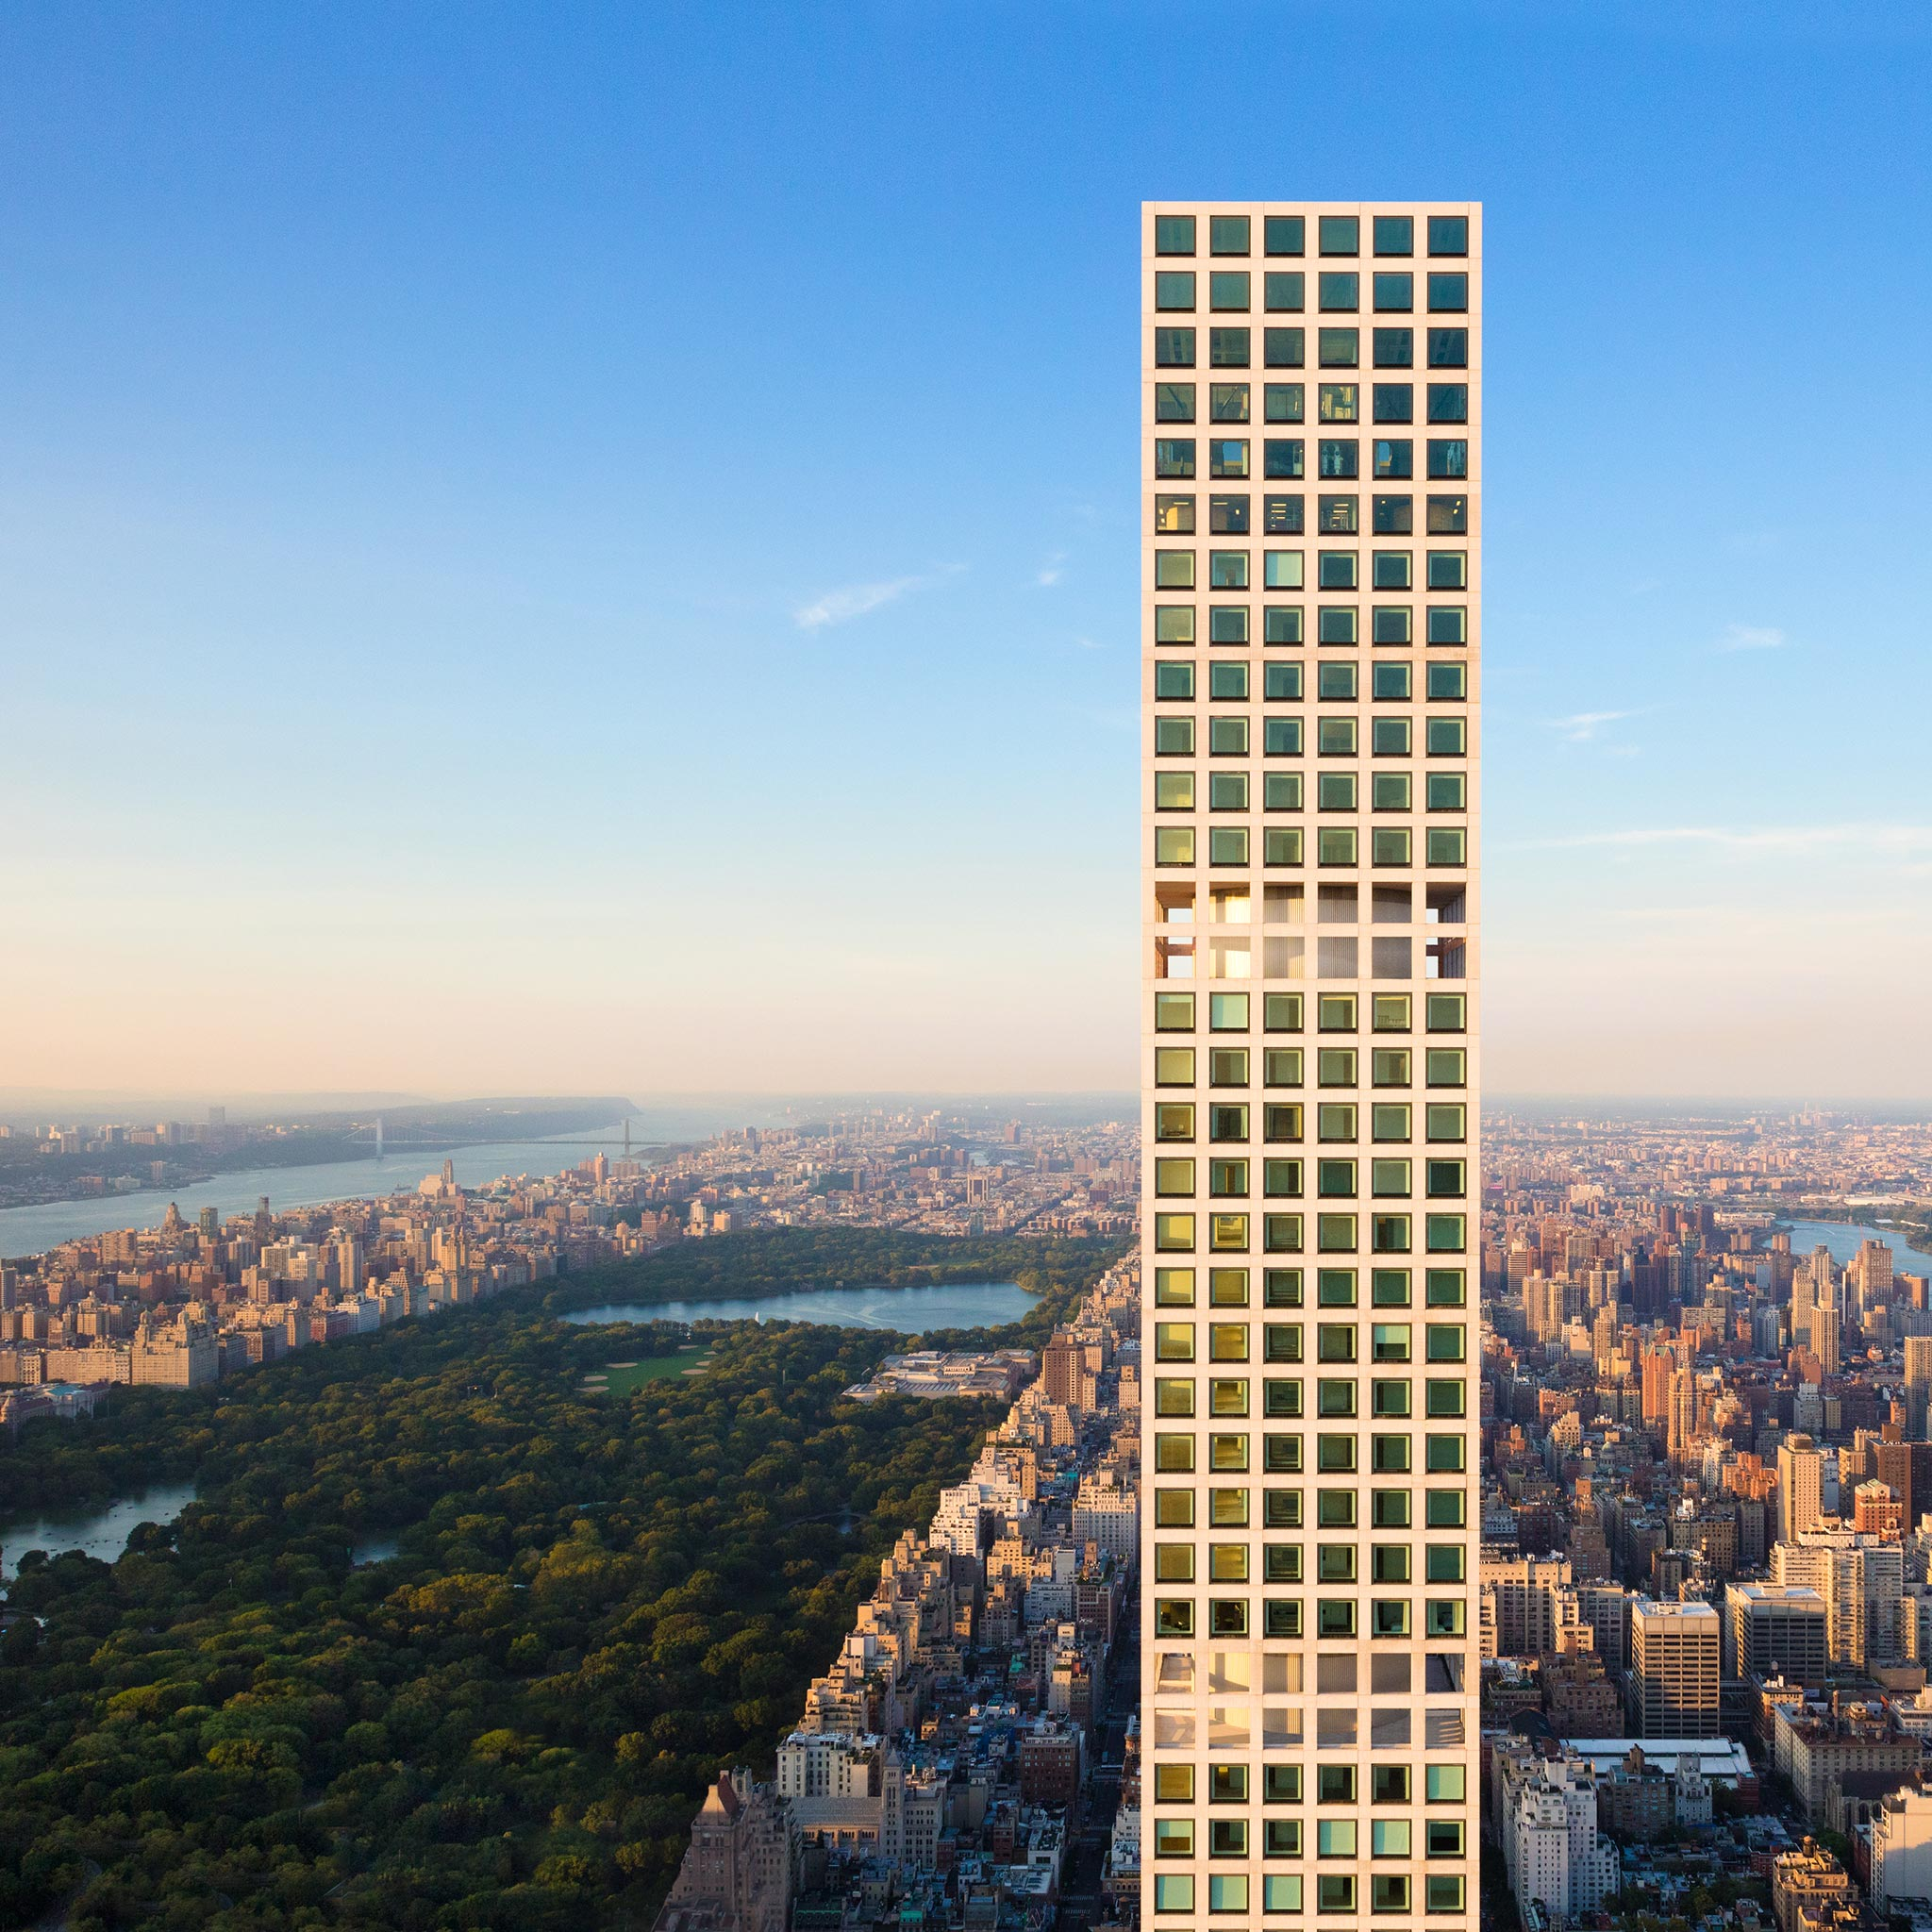
\includegraphics[width=\linewidth]{parkAvenue.jpg}

\end{figure}
\begin{table}[H]
\begin{tabular}{ll}
Name:				& Park Avenue 432\\
Höhe: 				& 426m\\          
Etagen:				% 88\\
Etagenhöhe:			4.72m\\
Hoechste Etage:		&392.1m\\
Wohnungen:			104\\
Speziell:			alle 12 Etagen 2 Etagen leer\\           
\end{tabular}
\end{table}
